% Hopefully this will be the final version of Problem statement.
\section{Problem Statement}

% \bx{What is Cloud computing and why it is the pillar of software and other related industry. (Importance of Cloud computing.)}
% \bx{
% \begin{itemize}
% 	\item (What) The main challenge for Cloud provider is to reduce energy consumption
% 	\item WHY it is important and SO WHAT? (consequences?),
% 	\item HOW to deal with it? (Technologies)
% \end{itemize}}

\bx{Cloud computing is a practice of using a network of servers to host softwares and data \cite{Mell:2011jj}}. It provides one of the most important utilities - computing power to the modern software industry \cite{2010arXiv1006.0308B}. With no upfront investment, low price and high availability (e.g services are accessible 99.99\% of the time), most web service providers such as Google and Neflix tend to deploy their services on Cloud. 

\bx{One of the challenges in Cloud computing is the huge energy consumption generated by data centers} - a typical data center consumes as much energy as 25,000 households \cite{Dayarathna:2016ua}. Since energy has become the major expense of cloud providers, cutting the energy bill becomes a critical mission which will lead to a cost reduction of softwares and consequently be beneficial to most people who access the Internet on a daily basis.

\bx{To reduce the energy consumption of a data center, the main target is to reduce the usage of physical machines (PMs) (e.g. servers).} Among several components in a data center such as cooling system, PMs, and network devices, PMs accounts for 40\% and have a huge improvement space. Currently, PMs always run in a low utilization as observed by Barroso and Shen \cite{Barroso:2007jt, Shen:2015hm} - from 10\% to 50\% of required resources on average.This is because cloud users tend to preserve more resources in order to guarantee the performance when facing the variation of workloads.

\bx{The major way to reduce the energy consumption of PM is through resource management \cite{Manvi:2014hm}.} Cloud resource management is a centralized system \cite{} that allocates resources to cloud users' applications, handles the workload fluctuations, and attempts to use as fewer number of PMs as possible to save energy. 

\bx{Currently, resource management in data centers \emph{virtualization} technology\cite{Uhlig:2005do}. } Such virtualization separates the resources (e.g. CPUs and RAMs) of a PM into several parts called \emph{virtual machines (VMs)}, each of which runs an isolated operating system. Before virtualization technology was widely used, traditional data center assigns a PM for each application; it causes the low utilization of PMs. Later on, when VMs are used to deploy applications, the utilization are largely improved and energy consumption are reduced. 

\bx{However, in recent years, the coarse resource management with VMs cannot catch up with a new trend in software industry - Service Oriented Architecture (SOA) \cite{Sprott:2004wt};} SOA is quickly becoming popular in modern software industry because of its agility and re-usability \cite{}. SOA separates a centralized application into multiple distributed components called web services. As most of web services only require a small amount of resources,  using a VM for a web service causes resource wastage inside a VM, consequently decreasing the utilization of PMs. 


\bx{In order to resolve the wastage inside VMs, a new virtualization technology: containers \cite{Felter:2015ki, Soltesz:2007cu} and a new service model: Container as a Service (CaaS) \cite{Piraghaj:2015uf} have been proposed to provide a finer granularity level of resource management.} Container is an operating system (OS) level of virtualization which run on top of VMs. CaaS uses containers as the fundamental resource management units. Thus, CaaS has the potential to improve the utilization of resources as well as energy consumption \cite{Esposito:2016br}. 



\begin{figure}
	\centering
	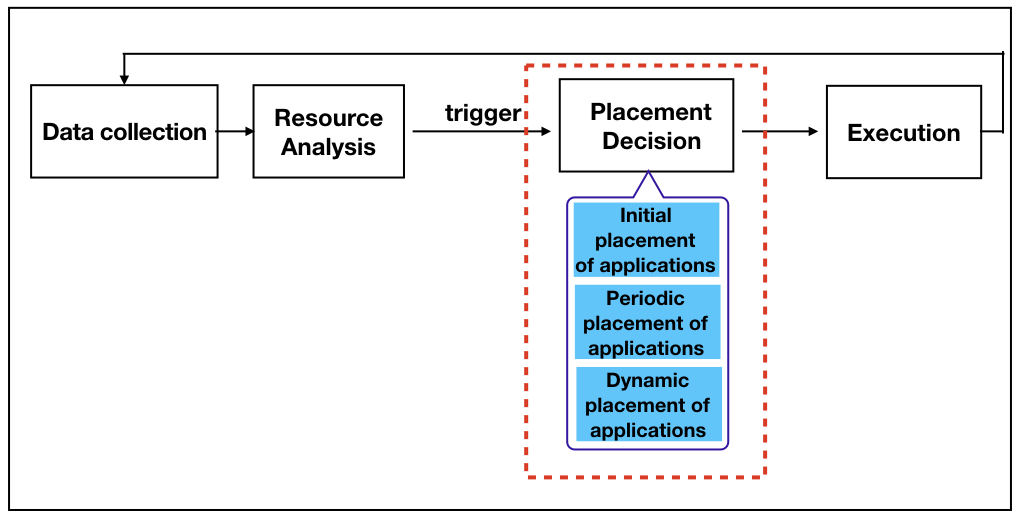
\includegraphics[width=0.7\textwidth]{pics/workflow_management.png}
	\caption{A workflow of resource management \cite{Mishra:2012kx}}
	\label{fig:workflow}
\end{figure}


\bx{Despite which virtualization is used, resource management includes four major steps \cite{Mishra:2012kx} (see Figure \ref{fig:workflow}): data collection, resource analysis, placement decision, and execution}. Among these steps, placement decision is the crucial step which includes three scenarios: application initial placement, periodic optimization and overloading & under-loading adjustment. In each scenario, server consolidation is a strategy to minimize the energy consumption.

% \bx{Although container technology gives an opportunity for better resource utilization, it also increases the difficulty of server consolidation.}
% Server consolidation \cite{Varasteh:2015fu} is an approach to efficiently use the resources of PMs in order to reduce the total number of PMs which leads to lower energy consumption. 

% \bx{Despite which virtualization is used, server consolidation can be applied in three resource management scenarios:} application initial placement  \cite{Jennings:2015ht}, periodic optimization \cite{Mishra:2012kx} and overloading/under-loading adjustments \cite{Mishra:2012kx} (see Figure \ref{fig:workflow}).

 % Server consumption is essentially an optimization task where it adjusts applications' locations in PMs so that a minimum number of PMs is used. For a certain number of applications, the fewer number of PMs is used, the less energy is consumed. 

% Three management processes: application initial placement, periodic optimization ,   have distinct characteristics, hence, the server consolidation techniques applied on them can be roughly classified into two categories: static \cite{Xiao:2015ik} and dynamic \cite{Beloglazov:2012bw}.

% \bx{In Initial application placement, the consolidation can be described as a static task conducted in an off-line manner.} 
\vspace{5mm}

\bx{Application initial placement is conducted when data centers receive a number of requests for new application deployment.}  The placement can be seen as a static optimization task where the optimization target is the locations of applications in PMs. 
% The optimization process can be described as: given a number of  PMs represented as resources (e.g CPU cores and RAM etc);  requested applications (wrapped with VMs or container) represented as aforementioned resources; the objective is to allocate these applications into a minimum number of PMs. The decision variable is the location of each application. The basic constraint is that the aggregative resources of hosted VMs cannot exceed the PM's resource capacity.
The placements in VM-based cloud and container-based cloud are different. In VM-based cloud, requested applications (wrapped with VMs) are placed into a minimum number of PMs. The problem is often modeled as a bin packing problem \cite{Xiong:2014jq}, with VMs represent items and PMs represent bins. The complexity is NP-hard \cite{Hochbaum:1996ts}. In a container-based Cloud, the optimization target expands to two levels - the lower level optimizes the placement of containers to VMs and the upper level optimizes the placement of VMs to PMs. These two levels of optimization is interact, therefore, it cannot be optimized separately. An additional constraint is that each container has its OS requirement which makes them cannot be simply packed into homogeneous VMs. Container-based placement can be seen as a bilevel optimization problem \cite{Colson:2007bu} where each level is bin packing problem. The hierarchy of bilevel optimization makes problems non-convex and strongly NP-hard \cite{Vicente:1994ie}.
% The placement problem in the VM context has been studied for years \cite{Xu:2010vh, Gao:2013gg, Ferdaus:2014ep} and it is often modeled as a bin packing problem . This is because VMs and PMs are naturally modeled as items and bins. Furthermore, server consolidation and bin-packing have the same optimization objective: minimize the number of bins/PMs. The complexity of bin-packing problem is NP-hard which is NP-hard \cite{Hochbaum:1996ts} which means it is extreme time-consuming to find its optimal solution when the number of decision variables is large. However, most research focus on VM-based server consolidation and these methods cannot be directly applied on container-based consolidation because of the different structure.




\bx{Only few research focus on container-based server consolidation problem. One of research is from Piraghaj and et al \cite{Piraghaj:2015uf}.} They propose a simple heuristics on two-step allocation, thus, did not consider the interaction between two levels (see detailed discussion in Section \ref{container-based-placement}). 
% In addition, their resource allocation system completely relies on dynamic placement without using static methods. Although their system can execute allocation fast, the energy efficiency cannot be guaranteed. 
Another research \cite{Mann:2016hx} is the earliest study which realizes two-level of placement should be considered together because they are interact with each other. They apply a fixed VM placement algorithm and considering a series of VM selection algorithms. The results also proves that the interaction between two placement cannot be ignored. 

\bx{In comparison of applying VMs and containers in initial application placement.} Containers have all the advantages of VMs such as live migration \cite{Clark:2005uda}, isolation of resource and performance. In addition, because containers offer a finer granularity level of resource management, it has the potential to further improve the utilization of resource which eventually reduces the energy consumption. 

\vspace{5mm}


% For the lower level of allocation, the objective is to maximize the utilization of resources (e.g a balanced utilization among several resources), while the upper level objective is to minimize the number of PMs. 
\bx{Periodic optimization takes existing applications' placement, re-placing them to PMs according to the nature of their workloads (e.g static, periodic or continuously changing etc).} Because the location of applications have been changed after this step, live migration technique is used to move one application from one PM to another. The live migration is a very expensive operation since it consumes network bandwidth and uses the resource on both host PM and target PM. Therefore, periodic optimization is a multi-objective task which considers minimizing the migration of applications and minimizing the overall energy consumption. 

\bx{Two major challenges exist in periodic optimization problem}. Firstly, it is a multi-objective task, two potentially conflicting objectives: reduce the number of migration and minimize the energy consumption. Therefore, the trade-off between two objectives must be balanced. Secondly, because of the expensiveness of live migration, cloud providers want to achieve a robust state of data center which means the placement remains stable in a long run. To achieve robustness, periodic optimization must consider the variation of workload and plan their position in advance. In literature, most research simply treat workload as a constant \cite{Viswanathan:2012ej, Chen:2011fl,Feller:2011vs}. According to Fehling \cite{Fehling:2014tl}, applications' workload are roughly classified into five categories: static, periodic, once-in-a-life-time, continuously changing, and unpredictable. Only a few research consider applying different strategies on different workloads. Meng et al \cite{Meng:2010gh} use a time-series analysis on workloads; they mapped complementary periodic workload as pairs and allocate them together. Their experiments showed promising results, however, they only mapped paired workloads which can be further improved by combining multiple workloads.
\vspace{5mm}


\bx{Overloading and underloading are scenarios which need an immediate reaction \cite{Beloglazov:2013ht}, thus, a dynamic placement is applied.}
Overloading is a scenario that the workloads exceed the capacity of its host PM. Hence, one or more applications will be migrated to other PMs. Underloading is when a PM runs in a low utilization, all the applications inside it will be moved to other PMs, so that the PM can be turned off. The common operation in these two scenarios are the dynamic placement \cite{Xiao:2015ik}. Dynamic placement places one application each time in an on-line manner. 

\bx{There are two challenges in this task.} On one hand, dynamic placement allocates an application at a time to meet the requirement of fast reaction. On the other hand, because it only considers the best allocation of the current application using either simple bin-packing algorithms such as First Fit or manually design heuristics. Simple bin-packing algorithms may perform poorly, as Mann's research \cite{Mann:2015ua} showed, server consolidation is a lot harder than bin-packing problem because of the multi-dimensional of resources, heterogeneous PMs, migration cost etc. While manual designed heuristics are designed for very specific scenarios, therefore, a single change of constraint may cause the failure of the algorithm. The second challenge is that, similar to periodic consolidation, different types of workload also need to be considered when dynamically matching the complementary workloads in order to reach a robust state.

% In addition, in container-based Cloud, the placement target is on containers and the destination is a suitable VM. However, if no VM can accommodate a container, a new VM must be created, which incurs a second level of deployment.

\bx{In summary, this thesis aims at improving the energy efficiency in a container-based cloud data center}. Specifically, we would like to address the major challenges in three resource management processes: application initial placement, periodic optimization and dynamic placement. The challenges are mainly focus on the optimization problem of two-level of placement problem and how to combine different types of workload to achieve high robustness.  
